\documentclass[12pt]{article}
\usepackage{xcolor}
\usepackage[latin]{babel}
\usepackage[utf8]{inputenc}
\usepackage[T1]{fontenc}
\usepackage{amsmath}
\usepackage{amsfonts}
\usepackage{amssymb}
\usepackage[version=4]{mhchem}
\usepackage{stmaryrd}
\linespread{1.5}
\setlength{\parindent}{0pt}
\usepackage{listings}
\usepackage{xcolor}
\usepackage{algorithm}
\usepackage{algpseudocode}
\usepackage{tikz}
\usepackage{pifont}
\usepackage{tikz}
\usetikzlibrary{positioning}  
\begin{document}

$\text{Q}_{1}$

PF:

As \textit{R}, \textit{$S_1$}, \textit{$S_2$}, \textit{T} aren't modified during the rotation, we only need to convince that \textit{v}, \textit{x}, \textit{s} are balanced after double rotation for the proof of the success of the rebalanced.

Let $r$ = size($R$), $s_1$ = size($S_1$), $s_2$ = size($S_2$), $t$ = size($T$)

$v$ is right-heavy, so either:

1. A node was added to $x$ to cause imbalance

2. A node was removed from $R$ to cause imbalance

Case I : a node was added to x to cause an imbalance

Assumptions:

$s_{1}+s_{2}+t+3>3(r+1) $   {\small\textcircled{\scriptsize{1}}}  
  $v$ is right-heavy 

$s_{1}+s_{2}+2 \leq 3(t+1) $   {\small\textcircled{\scriptsize{2}}} 
  $ x $ is balanced 
  
$\wedge t+1 \leq 3\left(s_{2}+s_{1}+2\right)${\small\textcircled{\scriptsize{3}}}

$s_{1}+1 \leq 3\left(s_{2}+1\right) $   {\small\textcircled{\scriptsize{4}}} 
  $ s$ is balanced 
  
$\wedge s_{2}+1 \leq 3\left(s_{1}+1\right)${\small\textcircled{\scriptsize{5}}}

$s_{1}+s_{2}+2 \geqslant 2(t+1)$   {\small\textcircled{\scriptsize{6}}} 
   assumption 
   

Before addition:


$3(r+1) \geq s_{1}+s_{2}+t+2$ {\small\textcircled{\scriptsize{7}}} $v$ was balanced

$\wedge r+1 \leq 3\left(s_{1}+s_{2}+t+2\right)$ {\small\textcircled{\scriptsize{8}}}

$\left.\begin{array}{l}
\left(t \leq 3\left(s_{1}+s_{2}+2\right)\wedge\left(s_{1}+s_{2}+2\right) \leq 3 t\right) \lor\\
\left(t+1 \leq 3\left(s_{1}+s_{2}+1\right)\wedge\left(s_{1}+s_{2}+1\right) \leq 3(t+1)\right)
\end{array}\right\} \Rightarrow \begin{array}{l}
t \leq 3\left(s_{1}+s_{2}+2\right)\text{\small\textcircled{\scriptsize{9}}} \\
\wedge\left(s_{1}+s_{2}+1\right) \leq 3(t+1)\text{\small\textcircled{\scriptsize{10}}}\end{array}$

$x$ was balanced

$\left.\begin{array}{l}
\left(s_{1} \leq 3\left(s_{2}+1\right) \wedge s_{2}+1 \leq 3 s_{1}\right) \lor \\
\left(s_{2} \leq 3\left(s_{1}+1\right) \wedge\left(s_{1}+1\right) \leq 3 s_{2}\right)
\end{array}\right\} \Rightarrow\begin{array}{l}s_{1} \leq 3\left(s_{2}+1\right) \text{\small\textcircled{\scriptsize{11}}}\\
\wedge s_{2} \leq 3\left(s_{1}+1\right)\text{\small\textcircled{\scriptsize{12}}}\end{array}$

$s$ was balanced

WTP:

$r+s_{1}+2 \leqslant 3\left(t+s_{2}+2\right)${\small\textcircled{\scriptsize{13}}} $s$ is balanced

$\wedge t+s_{2}+2 \leq 3\left(r+s_{1}+2\right)${\small\textcircled{\scriptsize{14}}}

$r+1 \leqslant 3\left(s_{1}+1\right)$ {\small\textcircled{\scriptsize{15}}} $v$ is balanced

$\wedge(s_1+1) \leqslant 3(r+1)${\small\textcircled{\scriptsize{16}}}

$s_{2}+1 \leq 3(t+1)${\small\textcircled{\scriptsize{17}}} $x$ is balanced

$\wedge(t+1) \leq 3\left(s_{2}+1\right)${\small\textcircled{\scriptsize{18}}}

By {\small\textcircled{\scriptsize{1}}}{\small\textcircled{\scriptsize{2}}}{\small\textcircled{\scriptsize{3}}}{\small\textcircled{\scriptsize{4}}}{\small\textcircled{\scriptsize{5}}}{\small\textcircled{\scriptsize{6}}}{\small\textcircled{\scriptsize{7}}}{\small\textcircled{\scriptsize{8}}}{\small\textcircled{\scriptsize{9}}}{\small\textcircled{\scriptsize{10}}}{\small\textcircled{\scriptsize{11}}}{\small\textcircled{\scriptsize{12}}}

We have:

$s_{1}+s_{2}+t+3>3(r+1)$ {\small\textcircled{\scriptsize{19}}}

$s_{1}+s_{2}+2 \leq 3(t+1)$ {\small\textcircled{\scriptsize{20}}}

$ t+1 \leq 3\left(s_{1}+s_{2}+2\right) ${\small\textcircled{\scriptsize{21}}}

$s_{1}+1 \leq 3\left(s_{2}+1\right)$ {\small\textcircled{\scriptsize{22}}}

$ s_{2}+1 \leq 3\left(s_{1}+1\right)${\small\textcircled{\scriptsize{23}}}

$ s_{1}+s_{2}+2 \geq 2(t+1) ${\small\textcircled{\scriptsize{24}}}

$ 3(r+1) \geq s_{1}+s_{2}+t+2${\small\textcircled{\scriptsize{25}}}

$ r+1 \leq 3\left(s_{1}+s_{2}+t+2\right) ${\small\textcircled{\scriptsize{26}}}

By {\small\textcircled{\scriptsize{19}}} {\small\textcircled{\scriptsize{20}}}: 

$ 3(r+1)<s_{1}+s_{2}+t+3=s_{1}+s_{2}+2+t+1 \leq 4(t+1) $

$ \Rightarrow r+1<\frac{4}{3}(t+1)<3(t+1)${\small\textcircled{\scriptsize{27}}}

Consider {\small\textcircled{\scriptsize{13}}}:

$
\begin{aligned}
r+ s_{1}+2=r+1+s_{1}+1 & <3(t+1)+3\left(s_{2}+1\right) \text { by {\small\textcircled{\scriptsize{22}}}, {\small\textcircled{\scriptsize{27}}} } \\
& =3\left(t+s_{2}+2\right) \text {, as wanted }
\end{aligned}
$

By {\small\textcircled{\scriptsize{25}}}

$3(r+1) \geqslant s_{1}+s_{2} + t+2>t+1$ {\small\textcircled{\scriptsize{28}}}

Consider {\small\textcircled{\scriptsize{14}}}:

$\begin{aligned}
t+s_{2}+2=t+1+s_{2}+1 & <3(r+1)+3\left(s_{1}+1\right) \text { by {\small\textcircled{\scriptsize{23}}} {\small\textcircled{\scriptsize{28}}} } \\
& =3\left(r+s_{1}+2\right) \text {, as wanted. }
\end{aligned}$

Consider {\small\textcircled{\scriptsize{15}}}:

$
\begin{aligned}
r+1&<\frac{4}{3}(t+1)  \text{by \small\textcircled{\scriptsize{27}}}\\
& =\frac{2}{3} \cdot 2(t+1) \\
& \leq \frac{2}{3}\left(s_{1}+s_{2}+2\right) \text { by \small\textcircled{\scriptsize{24}}} \\
& =\frac{2}{3}\left(s_{1}+1\right)+\frac{2}{3}\left(s_{2}+1\right) \\
& \leq \frac{2}{3}\left(s_{1}+1\right)+2\left(s_{1}+1\right) \text { by \small\textcircled{\scriptsize{23}}} \\
& <3\left(s_{1}+1\right)
\end{aligned}
$

$\Rightarrow r+1 \leq 3(s_1+1)$, as wanted

Consider {\small\textcircled{\scriptsize{16}}}:

$s_{1}+1  <s_{1}+s_{2}+t + 2 \leq 3(r+1)$ by {\small\textcircled{\scriptsize{25}}}

$\Rightarrow s_{1}+1  \leqslant 3(r+1)$ , as wanted 


Consider {\small\textcircled{\scriptsize{17}}}:

$s_{2}+1<s_{1}+s_{2}+2 \leq 3(t+1)$ by {\small\textcircled{\scriptsize{20}}}

$\Rightarrow s_{2}+1 \leqslant 3(t+1)$ as wanted

Consider {\small\textcircled{\scriptsize{18}}}:

$
\begin{aligned}
 t+1 &\leq \frac{1}{2}\left(s_{1}+s_{2}+2\right) \quad \text { by {\small\textcircled{\scriptsize{24}}}}  \\
&=\frac{1}{2}\left(s_{1}+1+s_{2}+1\right) \\
& \leq \frac{1}{2}\left(4\left(s_{2}+1\right)\right) \text { by {\small\textcircled{\scriptsize{22}}}} \\
&=2\left(s_{2}+1\right) \\
&<3\left(s_{2}+1\right) \\
& \Rightarrow t+1 \leq 3\left(s_{2}+1\right) \text { as wanted }
\end{aligned}
$

Therefore, $v.x.s$ are balanced after double rotation

Case II: a node was removed from $R$ to cause imbalance

Assumptions:

$s_{1}+s_{2} + t+3>3(r+1) {\small\textcircled{\scriptsize{29}}}\quad v$ is right-heavy

$s_{1}+s_{2}+2 \geqslant 2(t+1)$ {\small\textcircled{\scriptsize{30}}} assumption

Before removal:

$3(r+2) \geq s_{1}+s_{2}+t+3$ {\small\textcircled{\scriptsize{31}}} $v$ was balanced 

$\wedge r+2 \leq 3\left(s_{1}+s_{2}+t+3\right)$ {\small\textcircled{\scriptsize{32}}}

$s_{1}+s_{2}+2 \leq 3(t+1)$ {\small\textcircled{\scriptsize{33}}} $x$ was balanced 

$\wedge t+1 \leq 3\left(s_{2}+s_{1}+2\right)$ {\small\textcircled{\scriptsize{34}}} 

$s_{1}+1 \leq 3\left(s_{2}+1\right)$ {\small\textcircled{\scriptsize{35}}} $s$ was balanced 

$\wedge s_{2}+1 \leq 3\left(s_{1}+1\right)$ {\small\textcircled{\scriptsize{36}}} 

WTP:

$r+s_{1}+2 \leq 3\left(t+s_{2}+2\right)$ {\small\textcircled{\scriptsize{37}}} $s$ is balanced 

$\wedge t+s_{2}+2 \leq 3\left(r+s_{1}+2\right)$ {\small\textcircled{\scriptsize{38}}} 

$r+1 \leq 3\left(s_{1}+1\right)$ {\small\textcircled{\scriptsize{39}}} $v$ is balanced 

$\wedge\left(s_{1}+1\right) \leq 3(r+1)$ {\small\textcircled{\scriptsize{40}}} 

$s_{2}+1 \leq 3(t+1)$ {\small\textcircled{\scriptsize{41}}} $x$ is balanced 

$\wedge(t+1) \leq 3\left(s_{2}+1\right)$ {\small\textcircled{\scriptsize{42}}}

By {\small\textcircled{\scriptsize{29}}} {\small\textcircled{\scriptsize{33}}}

$3(r+1)<s_{1}+s_{2}+t+3=s_{1}+s_{2}+2+t+1 \leqslant 4(t+1)$

$\Rightarrow r+1<\frac{4}{3}(t+1)<3(t+1)$ {\small\textcircled{\scriptsize{43}}}

Consider {\small\textcircled{\scriptsize{37}}}:

$r+s_{1}+2=r+1+s_{1}+1 \leqslant 3(t+1)+3\left(s_{2}+1\right)=3\left(t+s_{2}+2\right)$
by {\small\textcircled{\scriptsize{35}}} {\small\textcircled{\scriptsize{43}}}

Consider {\small\textcircled{\scriptsize{38}}}:

$t+s_{2}+2 \leq s_{1}+s_{2}+t+2 \leq 3(r+2) \leq 3\left(r+s_{1}+2\right)
$ by {\small\textcircled{\scriptsize{31}}} 

Consider {\small\textcircled{\scriptsize{39}}}:



$$
\begin{aligned}
r+1& <\frac{4}{3}(t+1) \text{by {\small\textcircled{\scriptsize{43}}}}\\
& =\frac{2}{3} \cdot 2(t+1) \\
& \leq \frac{2}{3}\left(s_{1}+s_{2}+2\right) \text { by {\small\textcircled{\scriptsize{30}}}}  \\
& =\frac{2}{3}\left(s_{1}+1\right)+\frac{2}{3}\left(s_{2}+1\right) \\
& \leq \frac{2}{3}\left(s_{1}+1\right)+2\left(s_{1}+1\right) \text { by {\small\textcircled{\scriptsize{36}}}} \\
& <3\left(s_{1}+1\right)
\end{aligned}
$$

$\Rightarrow r+1 \leq 3(s_1+1)$, as wanted

Consider {\small\textcircled{\scriptsize{40}}}:

$3(r+1) \geqslant s_{1}+s_{2}+t$  {\small\textcircled{\scriptsize{44}}} by {\small\textcircled{\scriptsize{31}}}

 if $s_{2}+t=0$ 
 
As  $s_{2} \geqslant 0, t \geqslant 0$ ,

$ s_{2}=t=0$

$ s_{1}+2 \leq 3 \times 1$   by {\small\textcircled{\scriptsize{33}}}

$ s_{1} \leq 1 $

$ \therefore s_{1}=1$ or  0 

$ s_{1}+0+0+3>3(r+1) \geqslant 3$ by {\small\textcircled{\scriptsize{29}}}

$s_{1}>0 $

$ \Rightarrow s_{1}=1 $

$ 4>3(r+1)$  by {\small\textcircled{\scriptsize{29}}}

$3 r<1$

As $r \geqslant 0$,

$r=0$

$3(r+1) = 3 \geqslant 1=s_{1}+1$

else:

As $s_{2} \geqslant 0, t \geqslant 0$ and $s_{2}+t \neq 0, $

$ \Rightarrow s_{2}+t \geqslant 1 $

$\begin{aligned}
 3(r+1) &\geqslant s_{1}+s_{2}+t \quad \text { by {\small\textcircled{\scriptsize{44}}} } \\
&\geqslant s_{1}+1 
\end{aligned}$

$ \Rightarrow 3(r+1) \geqslant s_{1}+1 $

 By  two  cases:

$ 3(r+1) \geqslant s_{1}+1$

Consider {\small\textcircled{\scriptsize{41}}}

$s_{2}+1<s_{1}+s_{2}+2 \leq 3(t+1)$ by {\small\textcircled{\scriptsize{33}}}

$ \Rightarrow s_{2}+1 \leq 3(t+1)$ as wanted 


Consider {\small\textcircled{\scriptsize{42}}}

$$
\begin{aligned}
 t+1 &\leq \frac{1}{2}\left(s_{1}+s_{2}+2\right) \text {by{\small\textcircled{\scriptsize{30}}} }\\
&=\frac{1}{2}\left(s_{1}+1+s_{2}+1\right) \\
& \leq \frac{1}{2}\left(4\left(s_{2}+1\right)\right) \text {by{\small\textcircled{\scriptsize{35}}} }\\
&=2\left(s_{2}+1\right) \\
&<3\left(s_{2}+1\right) \\
& \Rightarrow t+1 \leq 3\left(s_{2}+1\right) \text { as  wanted} \\
\end{aligned}
$$

According to the two cases mentioned above,  $v.s.x$ are always balanced after double-rotation

$\Rightarrow$ In this case, the double counter-clockwise rotation restores the balance as wanted.

QED.

\newpage
$\text{Q}_{2}$

1.
\begin{verbatim}
split(T,k) -- pseudocode
  if T == nil:
      return (nil, nil, false) 
  if k == T.key:
      return (T.left, T.right, true)
  if k < T.key:
      (L, R, b) = split(T.left, k)
      T' = new node(key = T.key, size = 1, 
                    left = nil, right = nil)
      R_1 = join(R, T')
      R_2 = join(R_1, T.right)
      return (L, R_2, b)
  if k > T.key:
      (L, R, b) = split(T.right, k)
      T' = new node(key = T.key, size =1, 
                    left = nil, right = nil)
      L_1 = join(T.left, T')
      L_2 = join(L_1, L)
      return (L_2, R, b)
\end{verbatim}

2.
\begin{verbatim}
remove_max(T) -- pseudocode
  if T == nil:
      return (nil, none)
  if T.right == nil:
      return (T.left, T.key)
  (T.right, max) = remove_max(T.right)
  T.size -= 1
  T' = rebalance(T)
  return (T', max)
\end{verbatim}

\begin{verbatim}
join(L,G) -- pseudocode
  if L == nil:
      return G
  if G == nil:
      return L
  (L', max) = remove_max(L)
  T = new node(key = max, size = L.size + G.size,
               left = L', right = G)
  return rebalance(T)
\end{verbatim}

3.
\begin{verbatim}
difference(T_1, T_2) -- pseudocode
  if T_1 == nil:
      return nil
  if T_2 == nil:
      return T1
  k = T_2.key
  (L, R, b) = split(T_1, k)
  L' = difference(L, T_2.left)
  R' = differnece(R, T_2.right)
  return join(L', R')
\end{verbatim}

\newpage
$\text{Q}_{4}$

1.
\begin{table}[h]
    \centering
    \begin{tabular}{c|c}
        Node & is adjacent to \\ \hline
        1    & 2, 4, 3  \\
        2    & 5, 6   \\
        3    & 5, 7  \\
        4    & 6, 7   \\
        5    &       \\
        6    &       \\
        7    &       
    \end{tabular}
    \caption{Adjacency List for left tree}
\end{table}

\begin{table}[h]
    \centering
    \begin{tabular}{c|c}
        Node & is adjacent to \\ \hline
        1    & 4, 3, 2  \\
        2    & 5, 6   \\
        3    & 5, 7  \\
        4    & 6, 7   \\
        5    &       \\
        6    &       \\
        7    &       
    \end{tabular}
    \caption{Adjacency List for right tree}
\end{table}

2.

Suppose the given tree can be a breadth-first tree of $G$.

In this breadth-first tree, {3, 5} is a breadth-first tree edge. However, as 2 and 3 both can be the predecessor of 5, we need to dequeue 3 before 2 if we want to have {3, 5}. Now, 4 can either be before 3 or after 2 in 1's adjacency list. As 2 and 4 both can be the predecessor of 6 and we now have the breadth-first tree edge {2, 6}, 2 should be before 4. So, 4 can only be the last one in 1's adjacency list. Therefore, 3 is before 4 in  1's adjacency list and {3, 7} will be a breadth-first tree edge (the only two numbers that 7 is adjacent to are 3 and 4), which lets 4 be unable to be the predecessor of 7. But in the given tree, {4, 7} is a breadth-first tree edge while {3, 7} is not. There is a contradiction. So the supposition is false and the given tree cannot be a breadth-first tree of $G$.

\newpage
$\text{Q}_{5}$

The given problem can be converted into a problem that is coloring an undirected graph. Each wrestler can be considered as a vertex, and if two wrestlers are a pair of rivalry, then the two vertices that related to them have an edge between them. We need to color the two vertices of an edge with two different colors. So we need to generate an algorithm to color the graph's vertices with two different colors and return true if success, otherwise return false. We given each vertex a number to link it with the wrestler who has the same number. Then we will finally return an array A that A[i] is the
color of vertices i(i.e. the side we choose for the wrestler i, 0 is one side and 1 is the other).

\begin{verbatim}
bfs_color (start) -- pseudocode
  queue = new Queue()
  queue.enqueue(start)
  //define two colors are 0 and 1
  //define -1 means the vertices hasn't been colored
  start.color = 0
  while not queue.is_empty():
      u = queue.dequeue()
      for each v in u's adjacency list:
          if v.color == -1:
              queue.enqueue(v)
              v.color = 1 - u.color
          else if v.color == u.color:
              return false
  return true
\end{verbatim}

\begin{verbatim}
color_whole_graph (vertices_array) -- pseudocode
  for v in vertices_array:
      if v.color == -1:
          if bfs_color (v) == false:
              return false
  return true
\end{verbatim}

\begin{verbatim}
generate_solution (vertices_array, vertices_num) -- pseudocode
  if color_whole_graph(vertices_array):
      //it is possible to divide the wrestlers into two sides
      result[vertices_num]
      //set every elements in result be -1
      for i in range(n):
          result[i] = vertices_array[i].color
      return result
  // it is impossible to divide the wrestlers into two sides
  // no array to output
\end{verbatim}

bfs\_color (start) is an $O(n + r)$-time algorithm

color\_whole\_graph (vertices\_array) is also an $O(n + r)$-time algorithm

generate\_solution (vertices\_array, vertices\_num) is an $O(n)$-time algorithm

So the whole algorithm is $O(n + r)$.

\newpage
$\text{Q}_{6}$

1.
\[
\begin{array}{c|l}
a & b \rightarrow \cdot \\
b & a \rightarrow \cdot \\
c & b \rightarrow g \rightarrow \cdot \\
d & c \rightarrow \cdot \\
e & a \rightarrow f \rightarrow \cdot \\
f & a \rightarrow c \rightarrow \cdot \\
g & f \rightarrow h \rightarrow \cdot \\
h & d \rightarrow \cdot \\
\end{array}
\]

2.

$d(a) = 1, d(b) = 2, d(c) = 3, d(d) = 4$ 

$d(e) = 11, d(f) = 10, d(g) = 6, d(h) = 5$

$f(a) = 16, f(b) = 15, f(c) = 14, f(d) = 9$ 

$f(e) = 12, f(f) = 13, f(g) = 7, f(h) = 8$

$R = [a, b, c, f, e, d, h, g]$

3.

$[a, b], [c, g, f, h, d], [e]$

4.

$v_1=[a, b], v_2=[c, g, f, h, d], v_3=[e]$
\begin{center}
    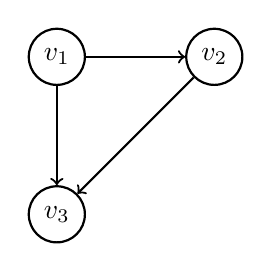
\begin{tikzpicture}[->, thick, node distance=2cm]

        % 定义带下标的节点
        \node (v1) [circle, draw] {$v_1$};
        \node (v2) [circle, draw, right of=v1] {$v_2$};
        \node (v3) [circle, draw, below of=v1] {$v_3$};

        \draw (v1) -> (v2);
        \draw (v1) -> (v3);
        \draw (v2) -> (v3);

    \end{tikzpicture}
\end{center}

5.

PF:

For a graph $G$, it has the same SCCs with its transpose graph.

Now we prove this statement. 

Consider an arbitrary SCC in $G$, we call it $C_1$. Then all the points in this SCC is reachable from each other. Suppose the points are $\{u_1, u_2, ...,u_n\}$. Consider two arbitrary vertices from this set $u_i, u_j$. We have path $p_i$ from $u_i $ to $u_j$ and path $p_j$ from $u_j $ to $u_i$. In $G^{T}$, as all the edge is reversed, the path $p_i$ and $p_j$ that are make up of several edges are also reversed in $G^{T}$. Let $p_i$ is reversed to $p_{i}'$ and $p_j$ is reversed to $p_{j}'$. Then $p_{i}'$ become the path from $u_j $ to $u_i$ and $p_{j}'$ become the path from $u_i $ to $u_j$. Thus, $u_i$ and $u_j$ are still reachable from each other in $G^{T}$. As $u_i$ and $u_j$ are arbitrary, all the point in $C_1$ are still reachable from each other in $G^{T}$. So $\{u_1, u_2, ...,u_n\}$ can still be in an SCC $C_{1}'$in $G^{T}$. Then we need to prove that $C_{1}'$ will not have more new vertices. We prove it from contradiction. Suppose there is a new vertex $w$ in $C_{1}'$. Therefore, $w$ and vertices in $\{u_1, u_2, ...,u_n\}$ are reachable from each other. We choose $w$ and an arbitrary $u_k(k\in\{1,2,...n\})$ to discuss. As in $G^{T}$,we have path $p_w$ from $w$ to $u_k$ and path $p_k$ from $u_k$ to $w$. In $G$, path $p_w$ will reverse and become the path from $u_k$ to $w$, and path $p_k$ will reverse and become the path from $w$ to $u_k$. This means $w$ and $u_k$ are also reachable from each other. As $u_k$ is arbitrary, $w$ and vertices in $\{u_1, u_2, ...,u_n\}$ are also reachable from each other in $G$. Then the SCC $C_1$ of $G$ is not the maximal subset of vertices reachable from each other in $G$, which is contradict to the definition of SCC. So our supposition is false and $C_{1}'$ will not have more new vertices. Then we have $C_1 = C_{1}'$. As $C_1$ is arbitrary, all the SCCs $C_t$ in $G$ will have a corresponding $C_{t}'$ in $G^{T}$ that have the same vertices. Finally, we have the statement that for a graph $G$, it has the same SCCs with its transpose graph as wanted.

Therefore, the component graphs of these two graph will have the same vertices. 

Consider an arbitrary edge $(v_{i}, v_{j})$ in $G^{SCC}$. 

Now we know that there is some vertex $u$ in $v_i$ has an edge to some vertex $v$ in $v_j$, and this edge will reverse to let the vertex $v$ in $v_j$ go to the vertex $u$ in $v_i$ if the graph $G$ transposes to $G^{T}$. This will cause $(G^{T})^{SCC}$ will have an edge $(v_{j}, v_{i})$. As the edge we choose is arbitrary, all the edge in $G^{SCC}$ will be reversed to be the new edge in $(G^{T})^{SCC}$ and no new edge will generate in $(G^{T})^{SCC}$, or the $G^{SCC}$ has to have the original reversed one. Therefore, $(G^{T})^{SCC}$ have the same vertices as $G^{SCC}$ and the edges are the reverse of $G^{SCC}$’s. This means $(G^{T})^{SCC}$ is the transpose of $G^{SCC}$ and also $G^{SCC}$ is the transpose of $(G^{T})^{SCC}$. Then we have $((G^{T})^{SCC})^T = G^{SCC}$ as wanted.

QED.

6.

The modified algorithm doesn't work. 

Suppose we start to visit a vertex $v_1$ whose SCC $C_1$ 
is linked by an edge from some vertex in another SCC $C_2$. Then the minimum discovery time in $C_2$ is larger than the minimum discovery time in $C_1$, as dfs($v_1$) will visit $C_1$ and the SCCs it link to first. Therfore, in the discovery time queue, the first vertex of $C_2$ is after the first vertex of $C_1$. So in the DFS($G^{T}$), we will visit $C_1$ first. However in the original graph $G$, $C_1$ is linked by an edge from some vertex in another SCC $C_2$, which means $C_1$ will linked to some vertex in $C_2$ in graph $G^{T}$. Thus, dfs($v_1$) will put both $C_1$ and $C_2$ in one SCC list. This is unacceptable, so the modified algorithm doesn't work.
\end{document}